\chapter{ADU}

\paragraph*{}
Die Benutzung des Analog-Digital-Wandlers (ADU) ermöglicht es Analoge Spannungen in digitale Werte umzuwandeln. Dies wird genutzt um Eingaben aus Analogschaltungen an den Controller zu übermitteln, etwa um Geräte anzuschließen, die Zustände in Spannungskurven codieren (z.B. Mikrophone).

\section{Aufgabe 23}

\paragraph*{}
In dieser Aufgabe soll der Wert einer externen Spannungsquelle gemessen werden und dann anschließend über die serielle Schnittstelle an den PC übermittelt werden. Zu erst initialisieren wir den Spannungswandler, und geben als obere bzw. untere Referenzspannung 3V bzw 0V an. Anschließend konfigurieren wir den Timer, so dass wir Abstand von einer Sekunde benachrichtigt werden. Die ISR signalisiert uns, wann wir eine Wandlung anstoßen sollen, dies minimiert den Code in der ISR. Allerdings kann dies dazuführen das wir eine neue Wandlung starten bevor die alte abgeschlossen ist (dieser Fall kann abgefangen werden, durch lesen des {\em ADC12BUSY}-Bits, welches angibt ob die Wandlung abgeschlossen wurde).

\lstinputlisting[caption=intterrupts.c für Aufgabe 23]{src/interrupts_aufgabe23.c}

\paragraph*{}
Als Ergebnis der Wandlung erhalten wir einen 12-bit langen Integer-wert. Dabei steht der Wert 4096 für unsere obere und 0 für die untere Referenzspannung. Dazwischen sind die Werte lineare verteilt. Durch eine einfache Rechnung erhalten wir den Wert in Volt und geben ihn anschließend auf der Konsole aus.

\lstinputlisting[caption=aufgabe23.c]{src/aufgabe23.c}

\section{Aufgabe 24}

\paragraph*{}
Im Hauptprogramm initialisieren wir den ADU und den TimerB um regelmäßig Wandlung durchzuführen. Dabei gehen wir weitgehend analog zu vorherigen Aufgabe vor. In der Endlosschleife warten wir auf einen Aufruf der Timer-ISR und starten eine Wandlung sobald diese uns signalisiert. 

\lstinputlisting[caption=aufgabe24.c]{src/aufgabe24.c}

\paragraph*{}
Wir nutzen die ISR des AD-Wandlers. Diese wird aufgerufen sobald die Wandlung abgeschlossen ist. Da der Prozessor über mehrere AD-Wandler verfügt können wir alle Werte auf einmal wandeln und diese anschließend auf die serielle Konsole schreiben.  

\lstinputlisting[caption=intterrupts.c für Aufgabe 23]{src/interrupts_aufgabe23.c}

\paragraph*{}
Als Ergebnis erhalten wir drei Kurven, die sich in Abhängigkeit von der Bewegung des Controllers ändern. Die z-Achse misst durchgehend höhere Werte, da sie die Erdbeschleunigung mit wahrnimmt.

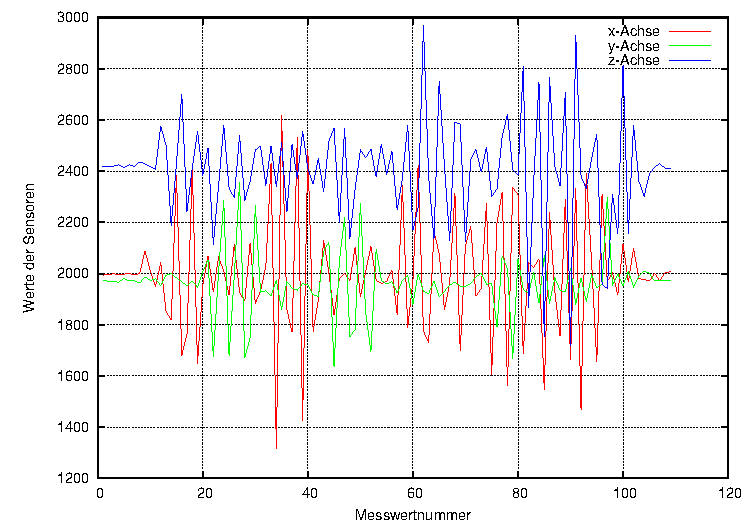
\includegraphics[width=\textwidth]{graphs/accel.pdf}

